\graphicspath{{literature_review/fig/}}

\chapter{Literature Review}
This chapter establishes the theoretical foundation for developing a low-cost impedance analyser for biosensing applications. The fundamental principles of biosensors and electrochemical impedance spectroscopy are examined, followed by an analysis of impedance measurement techniques and existing instrumentation approaches. This review identifies key design considerations and trade-offs that inform the development of a practical point-of-care impedance measurement system.
\section{Background on Biosensors}
Biosensors are employed in applications such as disease monitoring, drug discovery, and detection of pollutants, disease-causing micro-organisms and markers that are indicators of a disease in bodily fluids (blood, urine, saliva, sweat) \cite{bhallaIntroductionBiosensors2016}. 

% A biomarker is an objective measure that that gives an indication of the biological processes happening inside the body at a given moment \cite{BiomarkersNationalInstitute}. They are physical substances found in the body that can be measured. The concentration of biomarkers differs between healthy individuals and individuals with diseases, thereby aiding in diagnosis and monitoring of diseases \cite{rosenzweigWhatArePancreatic2018}. This project will focus on the development of a system that can be used for the detection of biomarkers found in blood samples. The concentration of these biomarkers in blood can give an indication of the presence and progression of a variety of diseases, including many types of cancer \cite{ribeiroApplicationsElectrochemicalImpedance2024}.


A biosensor consists of an analyte, a bioreceptor and a transducer mechanism combined with the electronics needed to process the signal \cite{bhallaIntroductionBiosensors2016}. The analyte is the substance of interest that needs detection. When the analyte is a subtance that acts as an objective measure that that gives an indication of the biological processes happening inside the body at a given moment, they are reffered to as biomarkers \cite{BiomarkersNationalInstitute}. Bioreceptors are molecules such as enzymes, cells, DNA or antibodies that specifically recognise and interact with the analyte. They produce a signal (in the form of light, heat, pH, charge or mass change, etc.) when they interact with the biomarker \cite{bhallaIntroductionBiosensors2016}. 
% Antibodies are produced by vertebrates as part of their immune response to foreign organisms or substances (called antigens). They are the most common biorecognition element used in biosensors \cite{zengRecombinantAntibodiesTheir2012}. Antibodies are Y-shaped cells that can be divided into two distinct regions. The top of the Y is variable and binds to a specific antigen depending on the amino acids present in this region. The amino acids present in the constant region (the bottom of the Y) is similar between different classes of antibodies (within the same species of animal) \cite{zengRecombinantAntibodiesTheir2012}. This constant region binds to the substrate of the biosensor during immobilization, leaving the variable region free to bind with antigens \cite{suedaAntibodyImmobilizationImmunosensing2022a}.
% \begin{figure}[ht]
%     \centering
%     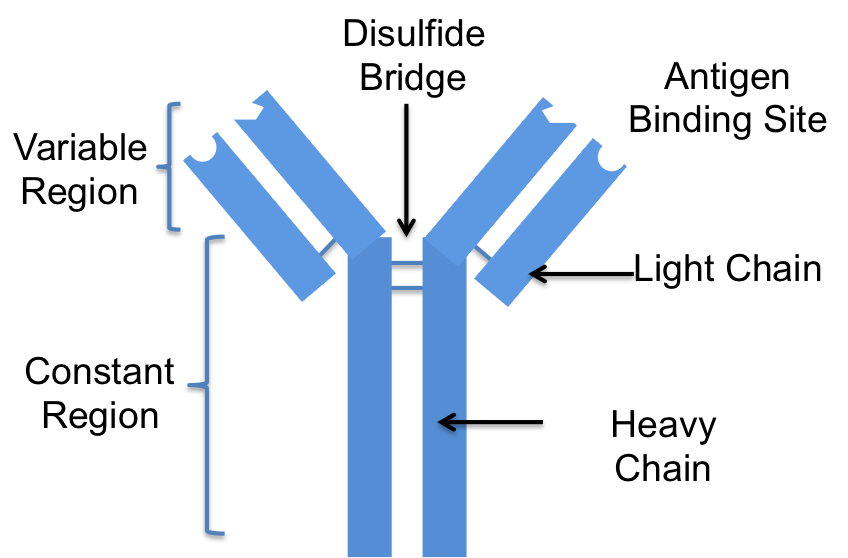
\includegraphics[width=0.7\textwidth]{antibody.png}
%     \caption[Antibody with basic structural features labeled]{Antibody with basic structural features labeled \cite{UsingAntibodiesVaccinea}}
%     \label{fig:antibody}
% \end{figure}

Many biosensors require that a "label" is attached to the biomolecule of interest and then the concentration of this label is detected and extrapolated to the concentration of the biomolecule \cite{danielsLabelFreeImpedanceBiosensors2007}. Label-free biosensors, on the other hand, directly detect the target biomolecule by measuring the changes in electrical properties of the surface of the biosensor when binding occurs. Since labelling can dramatically alter the binding properties of biomolecules and adds complexity and cost to the assay process, label-free detection is highly desirable \cite{danielsLabelFreeImpedanceBiosensors2007}, especially in point-of-care environments. The IDE's used for testing in this project use antibodies as the label-free bio-recognition element.

The concentration of the analyte in the sample can be estimated based on the number of bio-recognition events, however in order to convert the bio-recognition events into a measurable signal, a transducer mechanism is needed\cite{bhallaIntroductionBiosensors2016}. 

\subsection{Transducer Mechanisms}
There are various types of transducer mechanisms that can be used in biosensors, including optical, piezoelectric and electrochemical transducers. This project will focus on biosensors where binding events change the electrical properties of the biosensor, specifically the complex impedance. Thus, electrochemical transducers are of interest. 

Electrochemical transducers can use various analysis techniques. In potentiometric analysis, the potential of an electrode is measured against a reference electrode at zero-current \cite{magarElectrochemicalImpedanceSpectroscopy2021}. Coulometry applies a constant potential (with regard to a reference electrode) onto an electrode surface to carry out exhaustive electrolysis of an analyte \cite{magarElectrochemicalImpedanceSpectroscopy2021}. Voltammetry involves subjecting the sample to a varying potential at the electrode's surface and measuring the resulting Faradaic current \cite{magarElectrochemicalImpedanceSpectroscopy2021}. Finally, there is \ac{EIS}, which measures the complex impedance of an electrochemical system as a function of frequency \cite{magarElectrochemicalImpedanceSpectroscopy2021}. \Ac{EIS} is particularly suitable for biosensor applications where biological binding events alter the electrical properties of the electrode-electrolyte interface \cite{danielsLabelFreeImpedanceBiosensors2007}. 

\section{Fundamentals of EIS}
EIS involves applying a small sinusoidal perturbation to the \ac{DUT} and measuring the response. This can be either a voltage or current signal, \rephrase{while the other is measured}. By varying the frequency of the excitation signal, different electrochemical processes that occur at distinct time constants can be characterised.

\Ac{EIS} relies on the system acting as a linear time-invariant system, but most real-world electrochemical systems are inherently nonlinear \cite{lazanasErratumElectrochemicalImpedance2025}. To approximate linear behaviour and ensure valid results, EIS uses a small AC excitation signal, typically between 1–10 mVpp\cite{EISQualityIndicators}\cite{lazanasErratumElectrochemicalImpedance2025}. At higher amplitudes, the response deviates from ideal sinusoidal form, causing harmonic distortion and invalid measurements. However, making the excitation too small reduces signal-to-noise ratio, so 10 mVpp is commonly used to balance linearity and measurement quality.  
% Praat oor voordele van EIS bo ander metodes
A key advantage of \ac{EIS} is the ability to simulate the electrochemical system using equivalent circuit models. These models represent the various resistive, capacitive, and diffusive elements that represent the behaviour of the system \cite{lazanasErratumElectrochemicalImpedance2025}. This is due to the frequency domain nature of EIS, in comparison with other techniques such as voltammetry that works in the time-domain, thus allowing the behaviour of distinct processes that dominate at certain frequencies to be characterised \cite{lazanasErratumElectrochemicalImpedance2025}. By fitting experimental impedance data to these models, parameters such as charge transfer resistance and double-layer capacitance can be extracted, which correlate with biomolecular interactions occurring on the electrode surface \cite{danielsLabelFreeImpedanceBiosensors2007}. This capability makes \ac{EIS} a powerful tool for label-free biosensing applications. 

EIS biosensors can be categorized into two main types based on their transduction mechanism: faradaic and non-faradaic sensors.

\subsection{Faradaic vs Non-Faradaic EIS Sensors}
In faradaic measurements, charge transfers occur at the electrode-solution interface and redox reactions occur on the electrode surface \cite{xieReviewAdvancementsNanoscale2020a}. The basic equivalent circuit model for faradaic sensors is the Randles circuit (Figure \ref{fig:randles_fardaic}), consisting of solution resistance ($R_s$) in series with the parallel combination of double-layer capacitance ($C_{dl}$) and charge transfer resistance ($R_{CT}$) plus Warburg impedance ($Z_w$) representing diffusion processes \cite{xieReviewAdvancementsNanoscale2020a}.

Non-faradaic measurements operate without charge-transfer reactions, functioning as capacitive sensors that detect changes in the electrical double layer capacitance. Due to the lack of charge-transfer, $R_{CT}$ becomes infinitely large, thus creating an open circuit \cite{xieReviewAdvancementsNanoscale2020a}. On solid electrodes, the observed impedance response of $C_{DL}$ differs from an ideal capacitor, thus a \ac{CPE} is used instead of $C_{DL}$ in the Randles non-fardaic equivalent circuit (Figure \ref{fig:randles_non_faradaic}).  

\begin{figure}[ht]
    \centering
    \begin{subfigure}{0.45\textwidth}
        \centering
        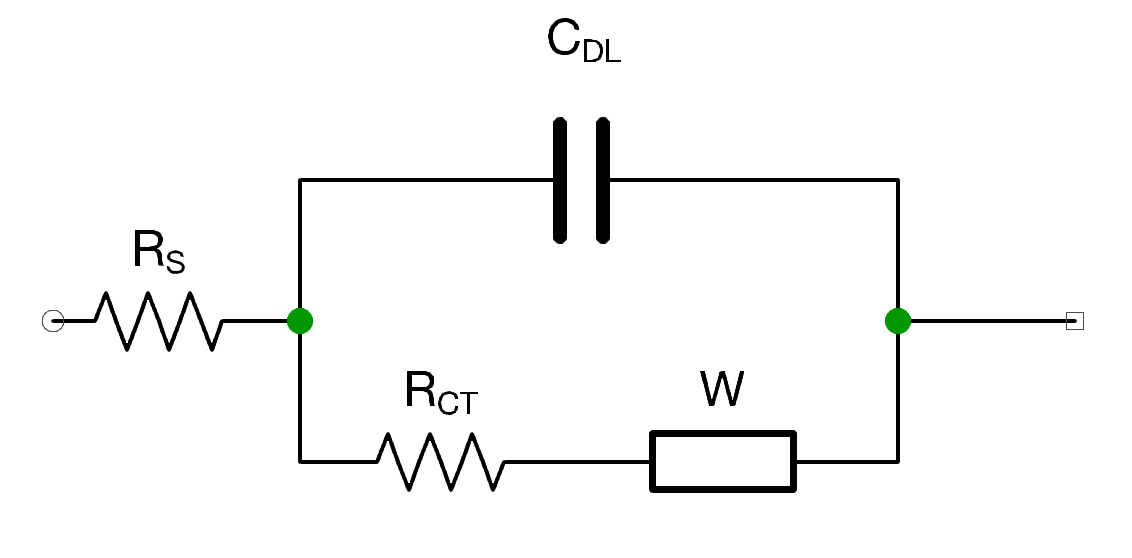
\includegraphics[width=\textwidth]{RandlesFaradaic.png}
        \caption{Faradaic Randles Circuit}
        \label{fig:randles_fardaic}
    \end{subfigure}
    \hfill
    \begin{subfigure}{0.45\textwidth}
        \centering
        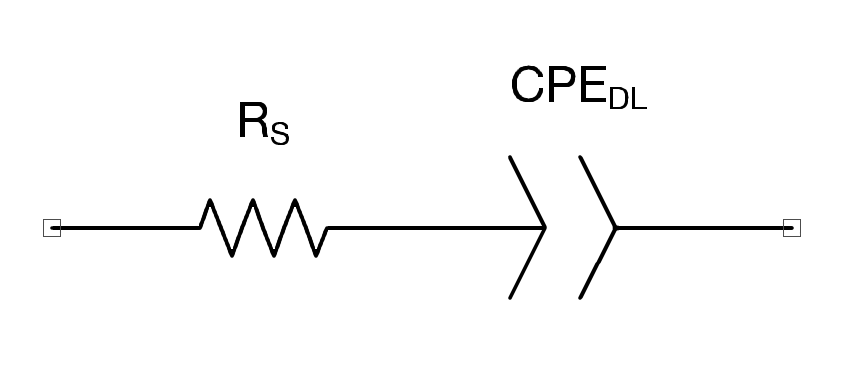
\includegraphics[width=\textwidth]{RandlesNonFaradaic.png}
        \caption{Non-Faradaic Randles Circuit}
        \label{fig:randles_non_faradaic}    
    \end{subfigure}
    \caption{Equivalent Circuits for Faradaic and Non-Faradaic EIS Biosensors}
    \label{fig:randles_circuits}
\end{figure}

\Ac{EIS} produces complex impedance data which contain both magnitude and phase information across a range of frequencies. \rephrase{This data is what allows for the characterisation of the electrochemical system and the extraction of parameters through equivalent circuit modelling.}

\section{Complex Impedance}
The complex impedance can be calculated as:
\begin{equation}
    Z(\omega) = \frac{V(\omega)}{I(\omega)} = Z'(\omega) + jZ''(\omega)
\end{equation}
where $Z'(\omega)$ is the real component representing resistive behaviour and $Z''(\omega)$ is the imaginary component representing capacitive or inductive behaviour (with $V(\omega)$ and $I(\omega)$ representing the phasor voltage and current respectively) \cite{lazanasErratumElectrochemicalImpedance2025}.

Two major ways of visualizing this complex impedance are the Nyquist and Bode representations, each highlighting different aspects of the electrochemical response.

\subsection{Nyquist Plot}
A Nyquist plot displays the negative imaginary part of impedance($Z''(\omega)$) versus the real part ($Z'(\omega)$) \cite{BodeNyquistPlot}. Each point on the plot corresponds to a particular frequency, though the frequency is not explicitly shown along the axes. For biosensing, high-frequency data points are located near the origin (low impedance), while low-frequency points are farther along the curve (high impedance). The Nyquist plot has the distinct advantage that some circuit parameters can be read directly form the plot \cite{BodeNyquistPlot}. 

A purely resistive impedance is represented as a point on the x-axis, as it has no imaginary component and is not frequency dependent. A purely capacitive impedance on the other hand is represented as a straight vertical line on the y-axis, as it has no real component and its imaginary component varies inversely with frequency \cite{BodeNyquistPlot}. The series combination of resistive and capacitive elements, thus result in a vertical line, offset from the y-axis. The parallel combination of resistive and capacitive elements, however result in a semicircular arc, as current flows though the path of least resistance \cite{BodeNyquistPlot}. At low frequencies, the capacitor acts as an open circuit resulting in the x-axis intercept (or diameter of the semi-circle) representing the magnitude of the resistive elements in the circuit. The series combination of a resistor and parallel resistor-capacitor thus results in a semicircular arc offset from the y-axis.

For simple electrochemical systems such as a Randles cell, the Nyquist plot appears as a semicircle (frequencies where charge transfer phenomena dominate) ending in a straight line tail (frequencies where mass transfer phenomena dominate) (Figure \ref{fig:randles_nyquist}) \cite{lazanasErratumElectrochemicalImpedance2025}. The series resistance ($R_s$) can be read directly from the x-axis intercept at high frequencies (closer to the origin), while the charge transfer resistance ($R_{CT}$) is given by the diameter of the semicircle in middle frequencies. At low frequencies, the Warburg impedance ($Z_w$) manifests as a 45-degree line due to diffusion-limited processes \cite{lazanasErratumElectrochemicalImpedance2025}, explaining the observed tail.

\begin{figure}[H]
    \centering
    \begin{subfigure}{0.45\textwidth}
        \centering
        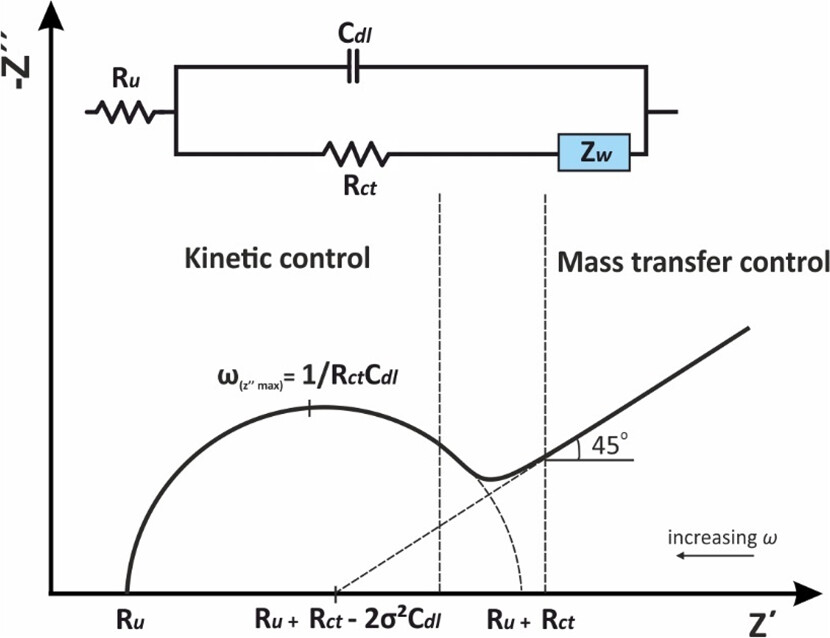
\includegraphics[width=\textwidth]{RandlesNyquist.jpeg}
        \caption[Faradaic Randles Circuit]{Faradaic Randles Circuit \cite{lazanasErratumElectrochemicalImpedance2025}}
        \label{fig:randles_nyquist_faradaic}
    \end{subfigure}
    \hfill
    \begin{subfigure}{0.45\textwidth}
        \centering
        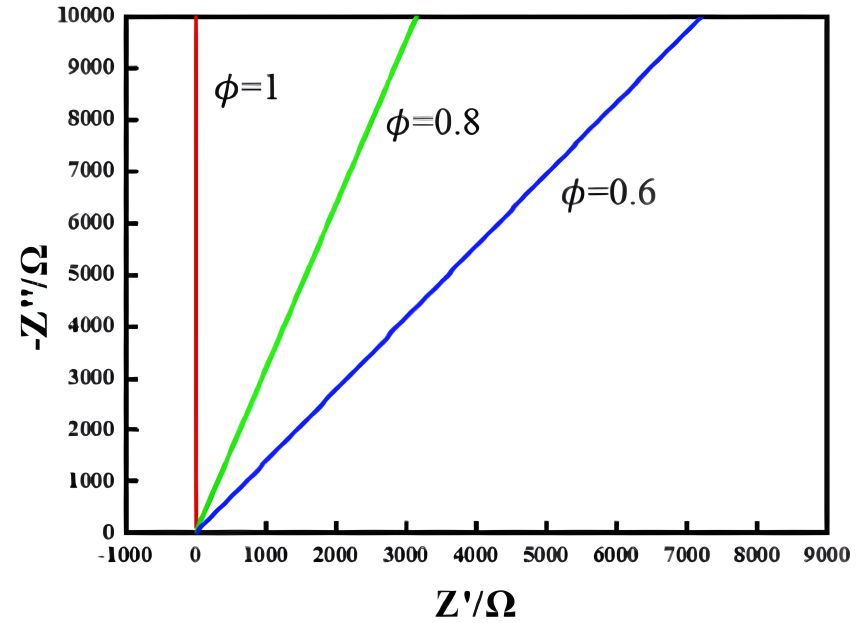
\includegraphics[width=\textwidth]{RandlesNonFaradaicNyquist.png}
        \caption[Non-Faradaic Randles Circuit]{Non-Faradaic Randles Circuit \cite{xieReviewAdvancementsNanoscale2020a}}
        \label{fig:RandlesNonFaradaicNyquist}    
    \end{subfigure}
    \caption{Nyquist Plots of Faradaic and Non-Faradaic Randles Circuits}
    \label{fig:randles_nyquist}
\end{figure}

The non-faradaic Randles equivalent, however does not exhibit a semi-circle, due to the exclusion of the charge transfer resistance ($R_{CT}$) and Warburg impedance ($Z_w$). Instead, the Nyquist plot appears as a straight line with an x-axis intercept representing $R_S$. For solid electrodes, however the line is not vertical as would be expected from the series combination of a resistive and purely capacitive element \cite{xieReviewAdvancementsNanoscale2020a} (Figure \ref{fig:RandlesNonFaradaicNyquist}). The $C_{DL}$ is thus replaced with a \ac{CPE} in the circuit model to account for this non-ideal capacitive behaviour.

\begin{equation}
    Z_{CPE} = \frac{1}{T(j\omega)^{\alpha}}
    \label{eq:cpe_impedance}
\end{equation}

The impedance of the \ac{CPE} is given by Equation \ref{eq:cpe_impedance}, with $\omega$ representing the angular frequency, $T$ being a constant related to capacitance, and $\alpha$ being an exponent between 0 and 1 that characterizes the deviation from ideal capacitive behaviour \cite{xieReviewAdvancementsNanoscale2020a}. $\alpha$ corresponds to the angle of the line in the Nyquist plot. When $\alpha = 1$, the \ac{CPE} behaves as an ideal capacitor, while values less than 1 indicate increasing non-ideality due to factors such as surface roughness or inhomogeneities \cite{xieReviewAdvancementsNanoscale2020a}.

An alternative representation of complex impedance data is the Bode plot.

\subsection{Bode Plots}

A Bode plot presents the magnitude, $|Z|$, and phase, $\phi$, of the impedance as functions of frequency on a logarithmic scale. The Bode magnitude plot reveals how impedance changes with frequency, while the phase plot shows the transition between capacitive ($\phi = -90^\circ$)  and resistive ($\phi = 0^\circ$) behaviour. While Nyquist plots offer direct visualization of resistive and capacitive interactions, Bode plots highlight the frequency dependence and allow clearer distinction of time constants \cite{BodeNyquistPlot}. In EIS analysis, both representations are complementary: Nyquist plots assist model-based fitting, whereas Bode plots verify consistency and highlight transition frequencies.

To obtain impedance measurements, specialised instrumentation known as impedance analysers are employed.

\section{Impedance Analysers}
\needscite{Impedance analysers integrate signal generation, voltage and current measurement, and data processing to determine the complex impedance of a \ac{DUT}. In biosensing, these devices perform \ac{EIS} by applying a known AC excitation and measuring the resulting voltage and current responses over a range of frequencies. The ratio of these phasor quantities provides the frequency-dependent impedance, revealing biochemical interactions at the electrode–electrolyte interface.}

Commercial solutions such as the PalmSens4, Gamry Reference 600+, and Metrohm Autolab PGSTAT offer exceptional accuracy, broad frequency ranges (typically 1 Hz to 1 MHz or higher), and advanced analytics including integrated equivalent circuit fitting. However, these instruments are prohibitively expensive ($\approx$ \texteuro 4200 for the PalmSens4) and require significant technical expertise to interpret results. This makes them unsuitable for low-resource \ac{POC} settings where portability, cost, and ease of use are crucial. Miniaturised, low-cost impedance analysers are therefore being actively developed for POC applications \cite{buscagliaSimpleZLowCostPortable2023, al-aliDesignPortableLowCost2017, ibrahimCMOSTransimpedanceAmplifier}. Such designs prioritise simplicity, automation, and affordability, while maintaining sufficient frequency range and measurement accuracy to detect biological binding events.

The analogue frontend of an impedance analyser typically consists of three main subsystems: signal generation, voltage measurement, and current measurement.
\subsection{Signal Generation}
\Ac{EIS} requires the generation of a small AC excitation signal, either voltage or current, to probe the \ac{DUT}. Generating a small current signal is difficult to do accurately and requires circuits such as the improved Howlard current pump \cite{ImprovedHowlandCurrent2020}. \needscite{On the other hand, generating voltage signals are simple, and thus the method commonly used in \ac{EIS} systems.}

Voltage-based signal generation can use dedicated chips like the AD5933 or custom solutions using microcontroller-based \acp{DAC}. The AD5933 offers integrated frequency sweeps and impedance measurement, making it attractive for simple implementations. However, it has several critical drawbacks. The chip has a DC offset between excitation and measurement stages, which is problematic because biosensing requires bipolar signals with no DC component. DC bias causes charge accumulation at the electrode–electrolyte interface, establishing a net electrochemical potential that drives unwanted redox reactions. Over time, these parasitic reactions alter the interfacial chemistry and change the electrode's impedance characteristics, obscuring the properties that \ac{EIS} aims to measure. The AD5933 also lacks direct voltage measurement capability and has a minimum measurable impedance of 1 k$\Omega$, further limiting its suitability for biosensing applications.

In contrast, a \ac{DAC} and \ac{ADC} solution implemented on a microcontroller allows precise control of excitation signals, flexible signal processing, and easier integration with multiplexing subsystems. 

When generating sinusoidal signals using a \ac{DAC}, the output is not a smooth analogue waveform but rather a series of discrete voltage steps. These steps introduce high-frequency components and harmonics not present in the original signal. Without filtering, they may interfere with downstream circuitry or cause aliasing during analog-to-digital conversion. An anti-aliasing filter (AA filter), typically a \ac{LPF}, is placed after the \ac{DAC} output to remove high-frequency content and smooth the signal.

The dynamic range of a \ac{DAC}, expressed in decibels, determines the smallest signal it can produce above its noise floor and is given by \cite{gaddyDYNAMICPERFORMANCETESTING}:
\begin{equation}
    \text{Dynamic Range} = 6.02n + 1.76 
    \label{eq:dac_range_lit}
\end{equation}
where $n$ is the number of bits of resolution. The AA filter must attenuate high-frequency components sufficiently so that aliased content falls below this noise floor, whilst maintaining a flat passband response to avoid distorting the intended output's amplitude or phase.

For systems generating signals across wide frequency ranges, a fixed-frequency AA filter becomes unsuitable. A single cutoff frequency cannot accommodate both low and high signal frequencies without either excessive attenuation or inadequate filtering. Variable AA filters address this by allowing dynamic cutoff adjustment. Many require changing resistor values to set the cutoff frequency, which is impractical for rapid frequency changes. Clock-tunable filters, which adjust their cutoff based on an external clock signal, thus offer a more flexible solution for wide frequency sweeps.

While some impedance analyser designs infer the applied voltage by using the known characteristics of the excitation stage \cite{buscagliaSimpleZLowCostPortable2023}, this fails to account for parasitic resistances, stray capacitance, drift, and environmental changes. Direct measurement captures all these variations, leading to reliable impedance calculations. This is vital in low-voltage biosensing where small changes significantly affect calculated impedance.

\subsection{Voltage Measurement}
Two common circuits for differential voltage measurements are differential op-amps and instrumentation amplifiers. Differential op-amps are simple and cost-effective but are susceptible to common-mode noise and offset errors \cite{technologyWhatAreDrawbacks2024}. They also have relatively low input impedance, which loads the signal source and affects measurements \cite{technologyWhatAreDrawbacks2024}. Instrumentation amplifiers are specifically designed for high-precision differential measurement. They provide superior common-mode rejection, high input impedance, and excellent accuracy even with small signals in noisy environments \cite{InstrumentationAmplifierOperational}. This is due to their three op-amp design, making them particularly suitable for biosensing where signals can be very small and minimising interference is critical.

Amplifying the measured voltage to fully utilise the \ac{ADC}'s linear range enhances both sensitivity and resolution. By maximising the voltage swing within the \ac{ADC}'s input range, the system can discriminate smaller changes in sensor response, allowing for better detection of low-concentration analytes. However, amplification introduces trade-offs related to gain-bandwidth product, which limits usable bandwidth at higher gains. Multi-stage amplification distributes gain across several stages, allowing higher overall gain whilst maintaining adequate bandwidth across the measurement frequency range.

While the measured voltage is relatively constant, the current through the \ac{DUT} can vary dramatically depending on its impedance. Thus, accurate current measurement is essential for determining the impedance of the \ac{DUT}.

\subsection{Current Measurement}
Two primary approaches to measuring current exist, namely shunt resistor based measurement and transimpedance amplifier based measurement.

The most basic method places a small known precision resistor (shunt resistor) in series with the current path and measures the voltage drop across it. Ohm's Law then gives the current. This approach is cheap and easy to implement but has severe drawbacks. The voltage drop across the resistor directly reduces the magnitude of the applied perturbation to the \ac{DUT}, impacting measurements. For biosensing, where signal levels are already low, even small drops significantly affect sensitivity.

A \ac{TIA} on the other hand, converts input current to a proportional output voltage without introducing significant voltage drop across the \ac{DUT}. The \ac{TIA} makes use of the following properties of op-amps:
\begin{equation}
    V_n \approx V_p
    \label{eq:opamp_V}
\end{equation}
\begin{equation}
    I_n \approx I_p \approx 0
    \label{eq:opamp_I}
\end{equation}
where $V_n$ and $V_p$ are the voltages at the inverting and non-inverting inputs respectively, and $I_n$ and $I_p$ are the input bias currents. The positive input (connected to the \ac{DUT}) is driven to the same potential as the negative input (ground or reference voltage), thereby ensuring a low-impedance path for the current. Conversely, Equation \ref{eq:opamp_I} ensures that the TIA has a high input-impedance and that the current from the sensor flows entirely through the feedback resistor. The output voltage is then given by:
\begin{equation}
    V_{out}=I_{in} \times R_{feedback}
    \label{eq:tia_gain}
\end{equation}
The \ac{TIA} has the advantage that unlike a shunt resistor, the feedback resistor can be large without affecting the applied signal.

In biosensing with fixed voltage perturbation, current varies dramatically depending on the \ac{DUT}'s impedance; from nanoamperes at high impedance to milliamperes at low impedance. A fixed-gain amplifier is impractical across this dynamic range. It would either saturate at high currents or provide insufficient resolution at low currents. Variable gain amplification, achieved through switchable feedback resistors in the \ac{TIA} or \acp{PGA} in subsequent stages, allows the system to adapt to current magnitude. This ensures output voltage remains within the optimal range for the \ac{ADC} whilst maximising measurement resolution.

\todo{Add linking sentence}

\section{Related Works}

\label{chap:literature_review}